\documentclass[11pt]{article}
\usepackage[T1]{fontenc}
\usepackage[utf8]{inputenc}
\usepackage{newtxtext}
\usepackage{newtxmath}
\usepackage[scaled=0.92]{helvet}
\usepackage{microtype}
\usepackage[a4paper,margin=1.4cm]{geometry}
\usepackage{tikz}
\usepackage{pgfplots}
\pgfplotsset{compat=1.18}
\usetikzlibrary{arrows.meta,positioning}
\usepackage[table]{xcolor}
\usepackage{enumitem}
\usepackage{multicol}
\usepackage{titlesec}
\usepackage{array}
\usepackage{booktabs}
\usepackage[hidelinks]{hyperref}

\definecolor{nbblue}{HTML}{1F4E79}
\definecolor{nbteal}{HTML}{2E8B8B}
\definecolor{nbred}{HTML}{B83227}
\definecolor{nbgrey}{HTML}{555555}
\definecolor{nbband}{HTML}{EAF0F6}

\setlength{\parindent}{0pt}
\setlength{\parskip}{2pt}
\titlespacing{\section}{0pt}{5pt}{2pt}
\titleformat{\section}{\sffamily\bfseries\color{nbblue}\normalsize}{}{0pt}{}
\setlist[itemize]{leftmargin=1.2em,itemsep=0.5pt,topsep=1pt,parsep=0pt}
\pagestyle{empty}
\renewcommand{\arraystretch}{1.12}

\newcommand{\hd}[1]{{\color{nbblue}\textbf{#1}}}

\begin{document}

%==================== TITLE ====================
\begin{center}
{\sffamily\bfseries\LARGE\color{nbblue} The Edge Negotiator}\\[3pt]
{\sffamily\large Coordinated On-Device SLMs for Multi-Junction Emergency Response}\\[5pt]
{\footnotesize\color{nbgrey} Progress report \,$\vert$\, MSc Systems Engineering for IoT, UCL (25153651) \,$\vert$\, Supervisors: Dr A.\ Delibasi (UCL), L.\ Stott (Microsoft) \,$\vert$\, 2026-06-21}
\end{center}
\vspace{2pt}
{\color{nbblue}\hrule height 1.2pt}
\vspace{8pt}

%==================== SCOPE ====================
\section{1.\ The project and its goal}
The system is a corridor of traffic junctions on one arterial. Its purpose is \textbf{coordinated emergency response}: when an ambulance crosses the corridor, or an incident blocks a lane, the junctions share what they see and clear a path together, instead of each reacting alone. Each junction runs a fast classical controller (\emph{MaxPressure}\,$^{[1]}$) by default, which is also the safety floor; a small AI model (\textbf{Phi-4-mini}, on the junction via \textbf{Microsoft Foundry Local}, never retrained) is called in only for the hard, ambiguous cases a fixed rule cannot settle.

Coordinating means acting on a neighbour's report, which is exactly what a compromised neighbour can abuse. So the enabling property, what makes the coordination safe to deploy, is \textbf{robust degradation}: if a junction is hijacked or its messages are tampered with, the system detects that the reports do not match the real traffic and falls back to local control. A deterministic safety net makes every clear-cut call (clear an ambulance a junction physically detects; refuse a claim it cannot verify); safety never depends on the AI. The central question we measure is whether the AI improves the genuinely ambiguous cases over a well-tuned fixed rule, and we report it either way.

%==================== TWO COLUMNS: diagram + chart ====================
\vspace{3pt}
\begin{minipage}[t]{0.50\textwidth}
\section{2.\ How it works}
\vspace{4pt}
\centering
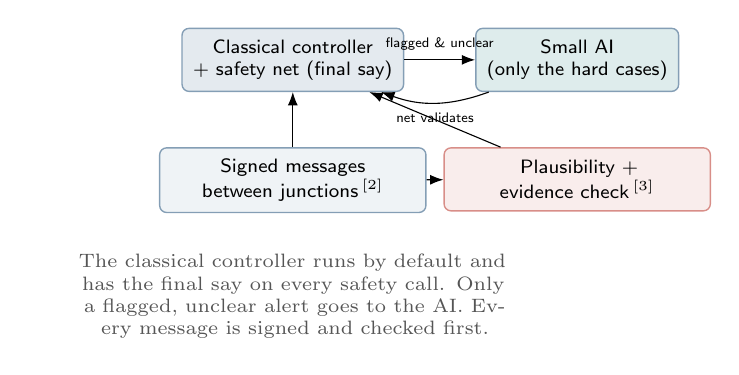
\begin{tikzpicture}[
  font=\sffamily\scriptsize,
  box/.style={draw=nbblue!55,line width=0.5pt,rounded corners=2.5pt,align=center,inner sep=4pt,minimum height=8mm},
  >=Latex]
\node[box,fill=nbblue!12] (mp) {Classical controller\\+ safety net (final say)};
\node[box,fill=nbteal!16,right=9mm of mp] (slm) {Small AI\\(only the hard cases)};
\node[box,fill=nbblue!7,below=7mm of mp,text width=3.1cm] (bus) {Signed messages\\between junctions\,$^{[2]}$};
\node[box,draw=nbred!55,fill=nbred!9,below=7mm of slm,text width=3.1cm] (gate) {Plausibility +\\evidence check\,$^{[3]}$};
\draw[->] (mp) -- node[above,font=\sffamily\tiny]{flagged \& unclear} (slm);
\draw[->] (slm) to[bend left=20] node[below,font=\sffamily\tiny]{net validates} (mp);
\draw[->] (bus) -- (mp);
\draw[->] (bus) -- (gate);
\draw[->] (gate) -- (mp);
\node[below=4mm of bus,font=\scriptsize,text width=6.5cm,align=center,color=nbgrey]
  {The classical controller runs by default and has the final say on every safety call. Only a flagged, unclear alert goes to the AI. Every message is signed and checked first.};
\end{tikzpicture}
\end{minipage}\hfill
\begin{minipage}[t]{0.47\textwidth}
\section{3.\ Measured effects (30 runs each)}
\vspace{4pt}
\centering
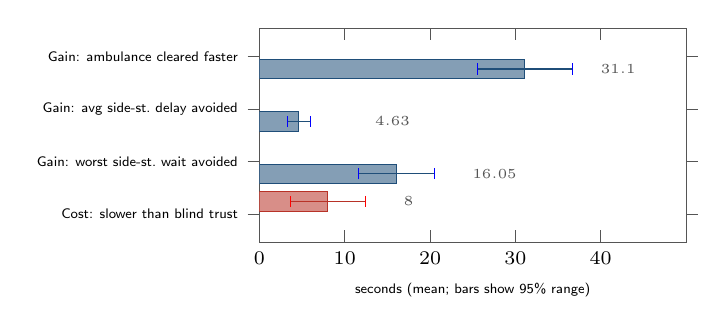
\begin{tikzpicture}
\begin{axis}[
  width=7.0cm,height=4.3cm,font=\sffamily\scriptsize,
  xbar,xmin=0,xmax=50,bar width=7pt,enlarge y limits=0.18,
  axis line style={nbgrey},tick style={nbgrey},
  xtick={0,10,20,30,40},
  xlabel={seconds (mean; bars show 95\% range)},xlabel style={font=\sffamily\tiny},
  ytick={0,1,2,3},
  yticklabels={Cost: slower than blind trust,Gain: worst side-st.\ wait avoided,Gain: avg side-st.\ delay avoided,Gain: ambulance cleared faster},
  yticklabel style={font=\sffamily\tiny,align=right},
  nodes near coords,
  nodes near coords style={font=\sffamily\tiny,color=nbgrey,anchor=west},
  every node near coord/.append style={xshift=24pt}]
\addplot+[draw=nbblue,fill=nbblue!55,error bars/.cd,x dir=both,x explicit] coordinates {
  (16.05,1)+-(4.47,0) (4.63,2)+-(1.37,0) (31.1,3)+-(5.55,0)};
\addplot+[draw=nbred,fill=nbred!55,error bars/.cd,x dir=both,x explicit] coordinates {
  (8.0,0)+-(4.39,0)};
\end{axis}
\end{tikzpicture}\\[2pt]
{\scriptsize\color{nbgrey} SUMO\,$^{[4]}$, 30 paired runs. Top: coordinated emergency preemption clears the ambulance faster than the same controller with preemption off. Below: the coordination stays safe under a spoofing neighbour, at a small honest cost. Every 95\% range excludes zero.}
\end{minipage}

%==================== PROGRESS ====================
\vspace{4pt}
\section{4.\ What we have built, and what it shows}
\begin{multicols}{2}
\begin{itemize}
\item \hd{Coordinated emergency handling (the core):} junctions share what they sense; a junction clears an ambulance it physically detects, and a downstream junction pre-clears for it once an upstream junction has independently confirmed the same vehicle.
\item \hd{Working and tested:} the classical controller and its safety net, signed messaging between junctions, an approved-senders registry, a check that flags neighbour reports inconsistent with the real traffic, and a four-junction simulated corridor.
\item \hd{Live demo:} a real ambulance is cleared across the junctions; a hijacked junction's signed-but-fake ``ambulance approaching'' alert is refused, so a compromised neighbour cannot hijack the coordination.
\item \hd{Evidence (30 runs):} coordinated emergency preemption (6 local plus 7 corroborated-downstream clearances in one run) clears the ambulance 31\,s faster than with preemption off; under a spoofing neighbour the worst side-street wait is held 16\,s below a trust-everything controller; requiring physical evidence costs 8\,s of ambulance time (accepted).
\item \hd{Independent check:} an automated audit of the write-up found no fabricated sources; a few over-stated citations were corrected. Every result is reproducible from its settings.
\end{itemize}
\end{multicols}

%==================== SURVEY ====================
\vspace{2pt}
\section{5.\ Where it sits in the literature}
To our knowledge, no prior system coordinates several junctions for emergency response using a frozen on-device SLM, and keeps that coordination trustworthy when an approved junction is compromised. The parts exist separately; this combination does not.

\vspace{4pt}
{\scriptsize\setlength{\tabcolsep}{4pt}
\rowcolors{2}{nbband}{white}
\begin{tabular}{>{\raggedright\arraybackslash}p{2.0cm} >{\raggedright\arraybackslash}p{4.7cm} >{\centering\arraybackslash}p{0.9cm} >{\centering\arraybackslash}p{0.9cm} >{\raggedright\arraybackslash}p{6.6cm}}
\rowcolor{nbblue!18}
\textbf{Work (year)} & \textbf{What it does} & \textbf{Coord?} & \textbf{Trust?} & \textbf{How we differ} \\
CoLLMLight (2025) & Cooperative LLM junctions share state; fine-tuned 8B & Yes & No & Frozen 3.8B; signed + plausibility-checked channel \\
VLMLight (2025) & Fast-classical + slow-LLM, safety-critical cases & 1 junc. & No & Multi-junction; small on-device model; compromised-channel test \\
LA-Light (2024) & LLM calls rule/RL for rare events; cloud GPT-4 & Multi & No & On-device; faults are adversarial and signed, not benign \\
iLLM-TSC (2024) & LLM refines an RL controller under noisy comms & No & Noise & Malicious (spoofed) messages, not random noise \\
LLMLight (2023/25) & Single LLM controls one junction; fine-tuned & No & No & Multi-junction coordination + trust layer \\
EMVLight (2022) & Trained MARL for emergency-vehicle preemption & Yes & No & No retraining; handles novel incidents; trust layer \\
REG-TSC (2025) & RAG + fine-tuned 8B agents, emergencies & Yes & No & Frozen 3.8B; RAG optional; signed + checked \\
CoLight (2019) & Graph-attention RL, cooperative control & Yes & No & Language reasoning on hard cases + security \\
MaxPressure (2013) & Throughput-optimal classical control & Local & No & Adopted directly as the default and safety floor \\
SafeLight (2023) & Trained RL + rule-based safety override & No & No & No training; defends against spoofed inputs \\
Blockchain-TSC (2019) & Blockchain secures vehicle$\rightarrow$signal data & No & Yes & Lightweight signed log; secures signal$\leftrightarrow$signal \\
proofmember23 (2023) & Device-identity / membership proof (IoT) & No & Yes & Applied to junctions + a content plausibility check \\
Derhab (2020) & Flow-conservation check for sensor-net attacks & n/a & Yes & Ported to vehicle conservation across junctions \\
Keijzer (2021) & Theory-only detection of coordination attacks & Yes & Yes & A measured detection-vs-attacker-strength curve; identity + audit \\
\end{tabular}}

\vspace{5pt}
\hd{Why this direction.} The contribution is the combination: a frozen on-device SLM coordinating several junctions for emergencies and incidents, kept safe when a junction is compromised. Coordination alone is precedented (CoLLMLight: normal flow, cloud-scale, fine-tuned, no trust); emergency handling alone is precedented (VLMLight, LA-Light, EMVLight); the fusion on a frozen edge model under a compromised channel is ours. Racing the classical controller on ordinary traffic is a dead end (throughput-optimal, microsecond-fast), so raw performance is a secondary, honest axis; the AI earns its place on the hard cases, and robustness to a lying neighbour is what makes leaning on a neighbour's report safe. We use SUMO (it models emergency vehicles and lane blockage), a signed hash-chained log not a blockchain (one trust domain), and a permissioned key registry not decentralised identity.

%==================== VALUE / KPIs ====================
\vspace{3pt}
\section{6.\ Value and how we measure success}
The deployable angle: a safety-critical demonstration of edge AI (Foundry Local, Phi-4, no cloud, no retraining) with verifiable agent identity, the same trust problem as Entra Agent ID, made physical and measurable. Success is judged on:

\vspace{3pt}
{\scriptsize\setlength{\tabcolsep}{5pt}
\rowcolors{2}{nbband}{white}
\begin{tabular}{>{\raggedright\arraybackslash}p{5.2cm} >{\raggedright\arraybackslash}p{12.4cm}}
\rowcolor{nbblue!18}
\textbf{Indicator} & \textbf{Target / acceptance} \\
Coordinated emergency-vehicle delay & Reduced versus the same controller with preemption off (measured: 31\,s faster over 30 runs); incident reallocation to follow \\
Spoofed-emergency resistance & Every uncorroborated emergency claim refused; no false preemption \\
No-harm guarantee & The security layer does not slow normal traffic beyond a pre-registered margin \\
Attack-detection quality & Precision / recall / detection-latency reported across a sweep of lie sizes \\
Edge feasibility & Phi-4-mini decision within budget on Foundry Local; gated to keep a corridor within it \\
Auditability & Tamper-evident log of every signed message and decision \\
\end{tabular}}

%==================== NEXT + HONESTY ====================
\vspace{2pt}
\begin{minipage}[t]{0.48\textwidth}
\section{7.\ Next steps}
\vspace{2pt}
\begin{itemize}
\item Central experiment: on flagged, unclear alerts, does the AI beat a well-tuned fixed rule? Measure and report either way, including a null.
\item Make normal-traffic coordination steer decisions, not only verify them, then measure the green-wave benefit.
\item Detection limit: grow the lie until detection fails; report where.
\item Real Euston Road (A501) arterial and a full demand sweep, with confidence ranges.
\item Run the real Phi-4-mini on Foundry Local; confirm repeatable decisions.
\end{itemize}
\end{minipage}\hfill
\begin{minipage}[t]{0.48\textwidth}
\section{8.\ What we do and do not claim}
\vspace{2pt}
{\footnotesize \textbf{Claim:} coordinated emergency preemption across junctions (a real ambulance cleared, a downstream junction pre-cleared on independent corroboration); authenticated messaging between junctions; detection of faked or faulty reports with a measured reliability curve; a deterministic safety floor; a fair attack-and-defence comparison.\\[3pt]
\textbf{Do not claim:} new cryptography; that the AI beats the classical controller on ordinary traffic; that the AI yet improves the ambiguous decisions (measured next); that normal-traffic green-wave coordination yet steers decisions (it is verified end to end but not yet causal, the next build step); defence against colluding insiders or a stolen master key; or that simulator results transfer directly to hardware.}
\end{minipage}

%==================== REFS ====================
\vspace{4pt}
{\color{nbblue!40}\hrule}
\vspace{2pt}
{\scriptsize\color{nbgrey}
\textbf{References.}\enspace
[1] Varaiya, Max-pressure control, \emph{Transp.\ Res.\ C} 36 (2013).
[2] Bernstein et al., Ed25519, \emph{J.\ Cryptogr.\ Eng.} (2012).
[3] Lighthill, Whitham \& Richards (LWR vehicle-conservation model, 1955, 1956).
[4] Lopez et al., SUMO, \emph{IEEE ITSC} (2018).
[5] Yuan et al., CoLLMLight, arXiv:2503.11739 (2025).
[6] Wang et al., VLMLight, arXiv:2505.19486 (2025).
[7] Wang et al., LA-Light, arXiv:2403.08337 (2024). Further: iLLM-TSC 2407.06025; LLMLight 2312.16044; EMVLight 2206.13441; REG-TSC 2510.26242; CoLight 1905.05717; SafeLight 2211.10871; Blockchain-TSC 1906.02628; proofmember 2310.08163; Derhab \emph{Sensors} 20(21):6106 (2020); Keijzer \emph{ECC} (2021).
}
\end{document}
